\documentclass[a4paper,11pt,twoside,onecolumn]{article}
\usepackage[a4paper,includehead,headsep=1mm,headheight=1pt,left=12mm,right=12mm,top=6mm,bottom=10mm,footskip=2mm]{geometry}
\title{myspectrogram.m}
\author{Kamil Wojcicki}

\usepackage[final]{mcode}
\usepackage[dvips]{graphicx}
\usepackage{epsfig}
\usepackage{color}
\usepackage{amsmath}
\usepackage{mathrsfs}
\usepackage{amsfonts}
\usepackage{amssymb}
\usepackage[dvips=true,bookmarks=true]{hyperref}
\usepackage{multirow}
\usepackage{multicol}
\usepackage{fancyhdr}
\usepackage{verbatim}
\usepackage{moreverb}
\usepackage{fancyvrb}
\usepackage{lscape}
\usepackage{longtable}
\usepackage{alltt}
\usepackage{xspace}
\usepackage{setspace}

\begin{document}
\maketitle
\pagestyle{plain}
\pagenumbering{arabic}

Usage:

\begin{enumerate}
\item Start Matlab
\item Run demo by typing: \texttt{test\_myspectrogram}
\end{enumerate}

\vspace{10mm}

\begin{figure}[ht!]
    \centering
    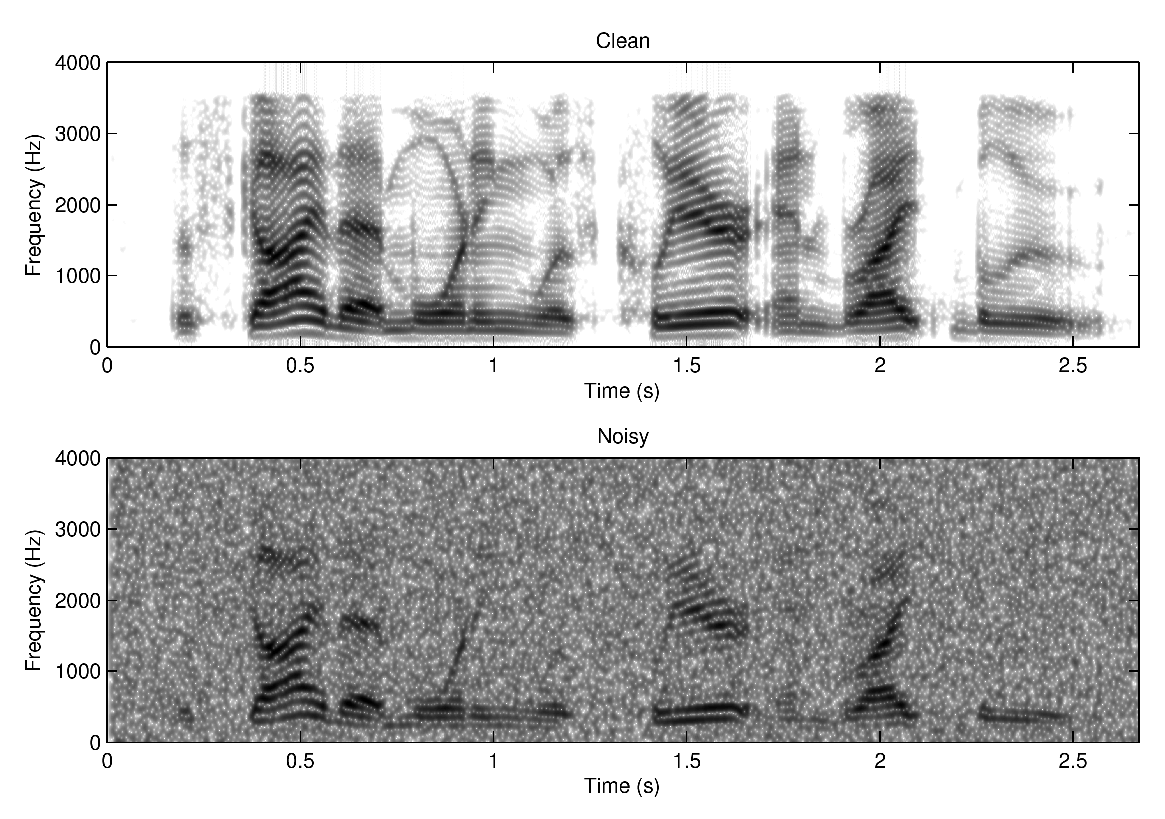
\includegraphics[width=0.7\linewidth]{test_myspectrogram.eps}
    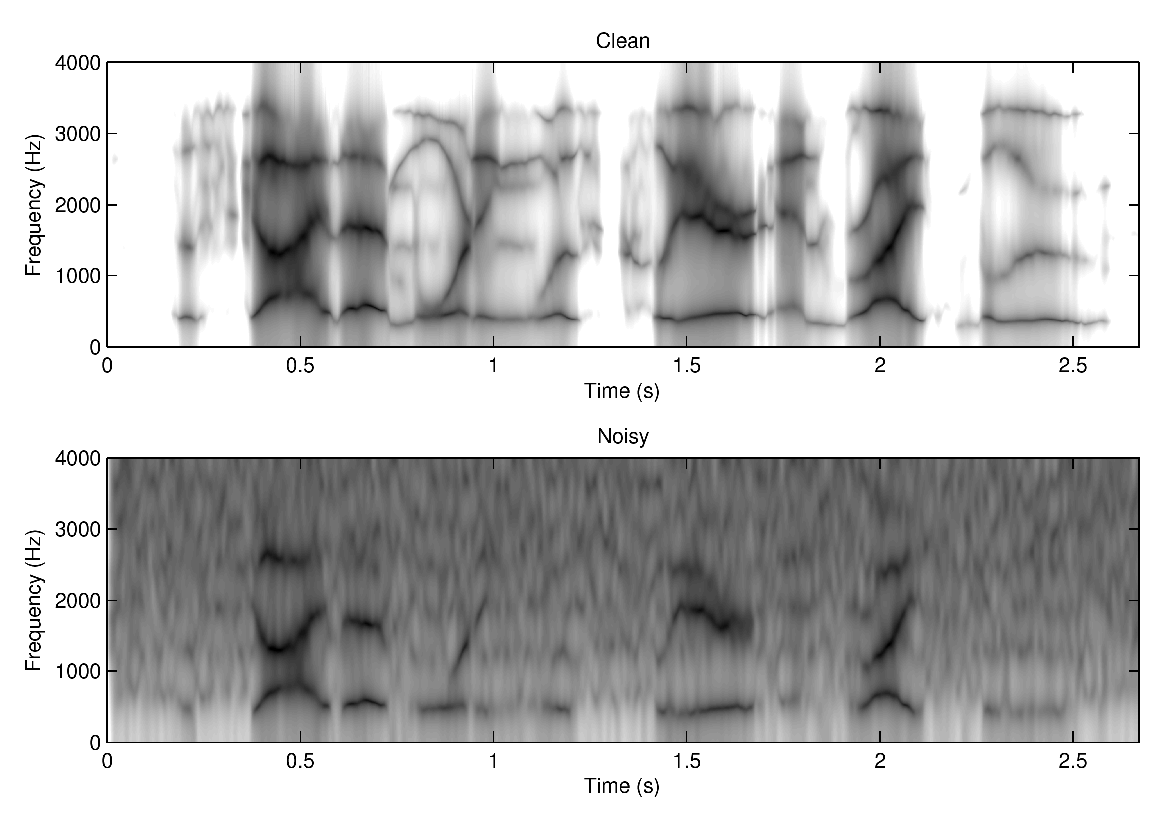
\includegraphics[width=0.7\linewidth]{test_myspectrogram_lp.eps}
\end{figure}
\clearpage

%\VerbatimInput[fontsize=\normalsize]{test_myspectrogram.txt}
%\vspace{10mm}

{\setstretch{1.05}\tiny\lstinputlisting{myspectrogram.m}}

\clearpage
{\setstretch{1.05}\tiny\lstinputlisting{test_myspectrogram.m}}

\end{document}	% EOF
